\documentclass[border=10pt]{standalone}
\usepackage{amsmath}
\usepackage{amssymb}
\usepackage{tikz}
\usetikzlibrary{arrows.meta,calc,decorations.pathreplacing,patterns,shapes.geometric,positioning,shadings,plotmarks}

\begin{document}
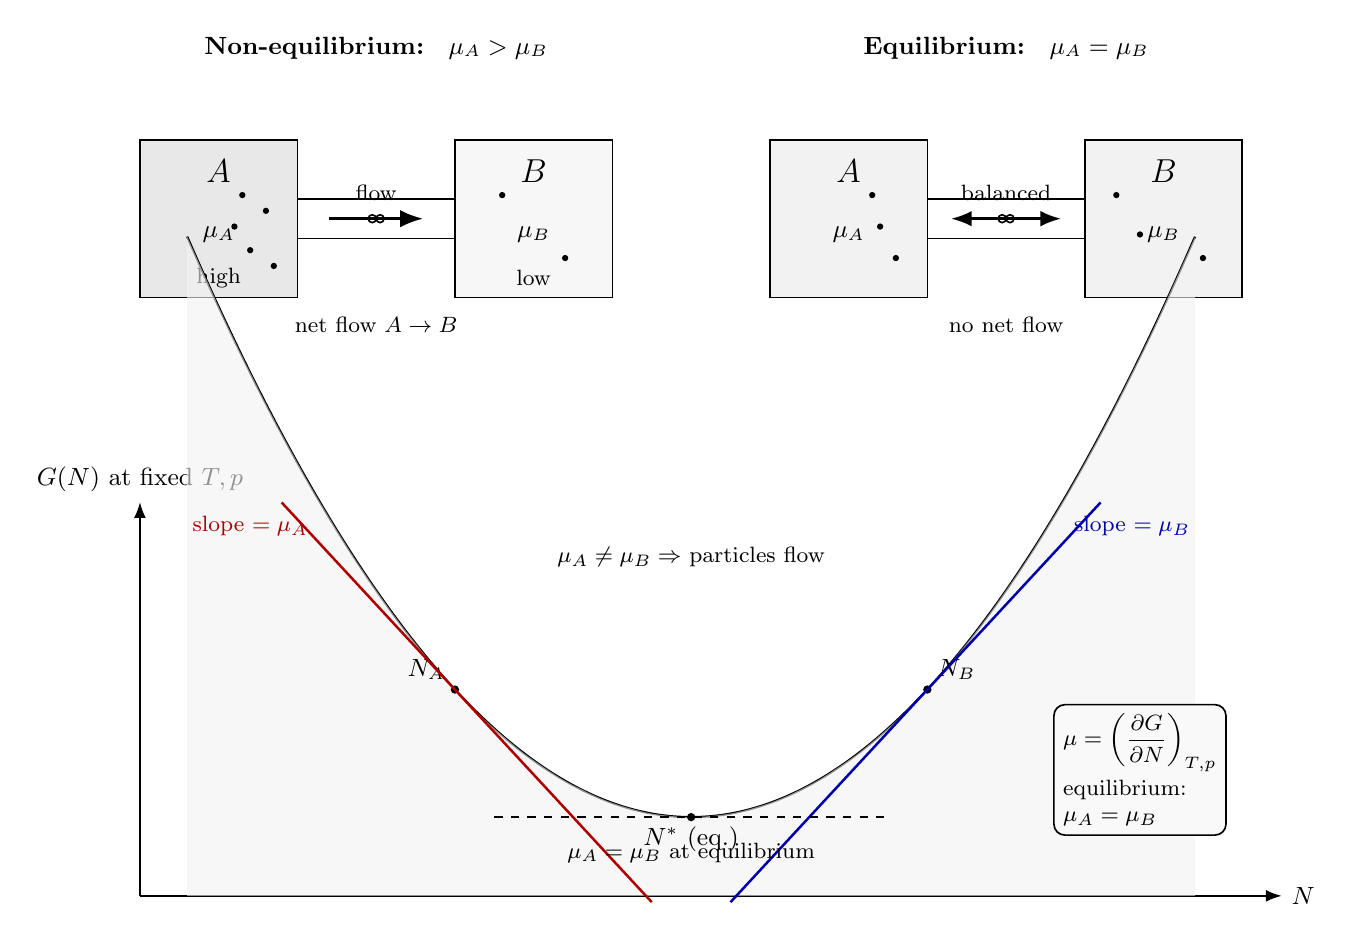
\begin{tikzpicture}[>=Latex, line width=0.6pt, font=\small]

% =========================================================
% TOP ROW: Two boxes A and B exchanging particles (two states)
% =========================================================

% --- LEFT SCENE: mu_A > mu_B  (non-equilibrium, net flow A -> B)
\begin{scope}[shift={(0,0)}]
  \node[anchor=south] at (3.0,3.5) {\textbf{Non-equilibrium: } $\mu_A > \mu_B$};

  % Box A (higher mu, light shading)
  \draw[fill=gray!18] (0.0,0.6) rectangle (2.0,2.6);
  \node at (1.0,2.2) {\large $A$};
  \node at (1.0,1.4) {$\mu_A$};
  \node[font=\footnotesize] at (1.0,0.85) {high};

  % Box B (lower mu)
  \draw[fill=gray!6] (4.0,0.6) rectangle (6.0,2.6);
  \node at (5.0,2.2) {\large $B$};
  \node at (5.0,1.4) {$\mu_B$};
  \node[font=\footnotesize] at (5.0,0.85) {low};

  % Connecting tube with small aperture
  \draw (2.0,1.85) -- (4.0,1.85);
  \draw (2.0,1.35) -- (4.0,1.35);
  % Small "hole" markers
  \draw[fill=white] (2.95,1.6) circle (0.05);
  \draw[fill=white] (3.05,1.6) circle (0.05);

  % Net particle flow A -> B (thick arrow)
  \draw[->, line width=1.2pt] (2.4,1.6) -- (3.6,1.6);
  \node[font=\footnotesize, above] at (3.0,1.7) {flow};

  % Tiny dots representing particles
  \fill (1.3,1.9) circle (0.04);
  \fill (1.6,1.7) circle (0.04);
  \fill (1.4,1.2) circle (0.04);
  \fill (1.7,1.0) circle (0.04);
  \fill (1.2,1.5) circle (0.04);

  \fill (4.6,1.9) circle (0.04);
  \fill (5.4,1.1) circle (0.04);

  % Label below
  \node[font=\footnotesize] at (3.0,0.25) {net flow $A \to B$};
\end{scope}

% --- RIGHT SCENE: mu_A = mu_B (equilibrium, balanced arrows)
\begin{scope}[shift={(8.0,0)}]
  \node[anchor=south] at (3.0,3.5) {\textbf{Equilibrium: } $\mu_A = \mu_B$};

  % Box A
  \draw[fill=gray!10] (0.0,0.6) rectangle (2.0,2.6);
  \node at (1.0,2.2) {\large $A$};
  \node at (1.0,1.4) {$\mu_A$};

  % Box B
  \draw[fill=gray!10] (4.0,0.6) rectangle (6.0,2.6);
  \node at (5.0,2.2) {\large $B$};
  \node at (5.0,1.4) {$\mu_B$};

  % Connecting tube
  \draw (2.0,1.85) -- (4.0,1.85);
  \draw (2.0,1.35) -- (4.0,1.35);
  \draw[fill=white] (2.95,1.6) circle (0.05);
  \draw[fill=white] (3.05,1.6) circle (0.05);

  % Balanced double arrow
  \draw[<->, line width=1.0pt] (2.3,1.6) -- (3.7,1.6);
  \node[font=\footnotesize, above] at (3.0,1.7) {balanced};

  % Dots roughly equal density
  \fill (1.3,1.9) circle (0.04);
  \fill (1.6,1.1) circle (0.04);
  \fill (1.4,1.5) circle (0.04);

  \fill (4.4,1.9) circle (0.04);
  \fill (5.5,1.1) circle (0.04);
  \fill (4.7,1.4) circle (0.04);

  % Label below
  \node[font=\footnotesize] at (3.0,0.25) {no net flow};
\end{scope}

% =========================================================
% BOTTOM: G(N) curve with two tangent lines
% =========================================================

\begin{scope}[shift={(0,-7.0)}]

  % Axes
  \draw[->] (0,0) -- (14.5,0) node[right] {$N$};
  \draw[->] (0,0) -- (0,5.0) node[above] {$G(N)$ at fixed $T,p$};

  % Convex curve G(N): use parabola-like shape (convex)
  % G(N) = 0.18*(N-7)^2 + 1.0  approximated via parabola
  \draw[thick, smooth, samples=80, domain=0.6:13.4]
    plot (\x, {0.18*(\x-7)*(\x-7) + 1.0});

  % Light shading under curve (region under G(N))
  \fill[gray!10, opacity=0.6]
    plot[smooth, domain=0.6:13.4] (\x, {0.18*(\x-7)*(\x-7) + 1.0})
    -- (13.4,0) -- (0.6,0) -- cycle;

  % --- Tangent at N_A (point with smaller slope, on the descending branch)
  % Choose N_A = 4: G' = 0.36*(4-7) = -1.08, G(4) = 0.18*9+1 = 2.62
  \coordinate (PA) at (4.0, 2.62);
  \fill (PA) circle (1.5pt);
  \node[above left] at (PA) {$N_A$};
  % Tangent line through PA with slope -1.08
  \draw[red!70!black, line width=0.9pt]
    ($(PA) + (-2.2, {-1.08*(-2.2)})$) -- ($(PA) + (2.5, {-1.08*2.5})$);
  \node[red!70!black, font=\footnotesize] at (1.4,4.7) {slope $= \mu_A$};

  % --- Tangent at N_B (point with larger slope, on the ascending branch)
  % Choose N_B = 10: G' = 0.36*(10-7) = 1.08, G(10) = 0.18*9+1 = 2.62
  \coordinate (PB) at (10.0, 2.62);
  \fill (PB) circle (1.5pt);
  \node[above right] at (PB) {$N_B$};
  \draw[blue!70!black, line width=0.9pt]
    ($(PB) + (-2.5, {1.08*(-2.5)})$) -- ($(PB) + (2.2, {1.08*2.2})$);
  \node[blue!70!black, font=\footnotesize] at (12.6,4.7) {slope $= \mu_B$};

  % Arrow indicating the slopes differ -> non-equilibrium
  \node[font=\footnotesize, align=center] at (7.0,4.3)
     {$\mu_A \neq \mu_B \Rightarrow$ particles flow};

  % --- Equilibrium illustration: two parallel tangents (same slope)
  % We mark a horizontal common tangent at the minimum (slope = 0) on
  % two symmetric points, but the shape is single-well so we instead
  % draw two parallel dashed tangents at slope 0.36 to illustrate
  % "equal slopes" condition
  % Equal-slope points: pick slope s = 0.36 -> 0.36*(N-7) = 0.36 -> N = 8
  % Only one point on this curve at slope 0.36; for visual we add the
  % minimum point with slope 0 as the equilibrium tangent.
  \coordinate (PEQ) at (7.0, 1.0);
  \fill (PEQ) circle (1.5pt);
  \node[below] at (PEQ) {$N^*$ (eq.)};
  \draw[dashed, line width=0.8pt] (4.5,1.0) -- (9.5,1.0);
  \node[font=\footnotesize] at (7.0,0.55) {$\mu_A = \mu_B$ at equilibrium};

  % Formula box
  \node[draw, rounded corners, fill=gray!5, font=\footnotesize, align=left]
    at (12.7,1.6)
    {$\mu = \left(\dfrac{\partial G}{\partial N}\right)_{T,p}$ \\[2pt]
     equilibrium: \\
     $\mu_A = \mu_B$};

\end{scope}

\end{tikzpicture}
\end{document}
